\documentclass{book}
\usepackage{graphicx}
\usepackage{amsmath}
\usepackage{amsfonts}
\usepackage{musicography}
\usepackage[dvipsnames]{xcolor}

\newtheorem{definition}{Definition}
\newcommand{\muskern}{\kern-.15ex }
\makeatletter
\newcommand\dynmark[1]{{\normalfont\bfseries\itshape
  \@tfor\next:=#1\do{\put@muskern\next}\/}}
\newcommand{\put@muskern}{\let\put@muskern\muskern}
\makeatother

\begin{document}
    \chapter{Notation}
    \section{Pitch}
\begin{definition}[Pitch]
    Pitch is the property of the sound which allows a relative ordering of perceived sounds on a frequency-related scale.
\end{definition}
On a keyboard, pitch goes up to the right of the keyboard, while it goes down on the left.

Pitches are expressed through \textbf{notes}. There are 7 note names\footnote{C-B in anglophone countries, C-H in Germany and Do-Si for the rest of Europe.}, which are repeated in \textbf{octave registers}, identified by the bottom number.
$$\cdots A_3 B_3 \underbrace{C_4 D_4 E_4 F_4 G_4 A_4 B_4}_{\text{Octave register 4}} C_5 D_5 \cdots$$

\begin{figure}[h]
    \begin{center}
        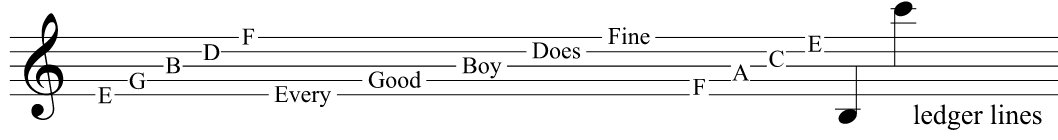
\includegraphics[width=0.8\textwidth]{img/treble}
        \caption{Treble clef}
        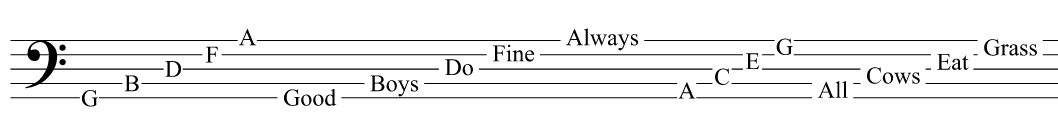
\includegraphics[width=0.8\textwidth]{img/bass}
        \caption{Bass clef}
    \end{center}
\end{figure}

\begin{definition}[Octave]
    The distance / interval between two notes with the same name.
\end{definition}

\begin{definition}[Middle C]
    The $C_4$ pitch, usually located in the middle of a keyboard (on the instrument) and always annotated in the middle of the grand staff, shared by the two staves.
\end{definition}

\begin{figure}[t]
    \begin{center}
        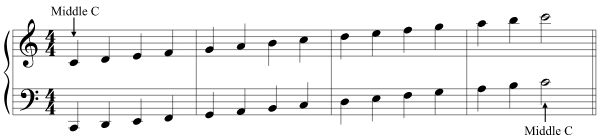
\includegraphics[width=0.8\textwidth]{img/grandstaff}
        \caption{The Grand Staff (a specific stave \emph{system})}
    \end{center}
\end{figure}

\begin{definition}[Accidental]
    A symbol placed before a note to raise / lower its pitch by a given amount.
\end{definition}

An accidental is effective only for a measure. They affect the entire piece if they are placed before the clef in a \textbf{key signature}.
\begin{center}
    \begin{tabular}{r|c|l}
        $\flat{}$ & Flat & $-1$ half step \\
        $\sharp{}$ & Sharp & $+1$ half step \\
        $\musDoubleFlat$ & Double flat & $-2$ half steps / $-1$ whole step \\
        $\musDoubleSharp$ & Double sharp & $+2$ half steps / $+1$ whole step \\
        $\natural{}$ & Natural & Cancels preceding accidentals \\
    \end{tabular}
\end{center}
There exists also \textbf{half-accidentals}, whose altered notes cannot be played on a keyboard.

\begin{definition}[Half step]
    On the keyboard, the distance / interval between one key (either black or white) and the next (either black or white).
\end{definition}

\begin{definition}[Whole step]
    The interval made up of two half steps.
\end{definition}

\begin{figure}[h]
    \begin{center}
        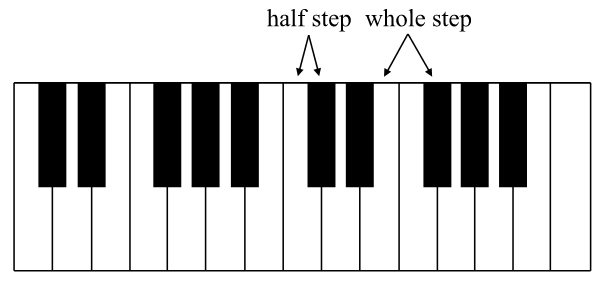
\includegraphics[width=0.6\textwidth]{img/halfstep}
        \caption{Half steps and whole steps}
    \end{center}
\end{figure}

\begin{definition}[Enharmonic]
    Which has the same sound, but different name.
\end{definition}

\section{Rhythm}
\begin{definition}[Beat / pulse]
    The basic pulse underlying measured music and thus the unit by which musical time is reckoned.
\end{definition}

\begin{definition}[Tempo]
    Speed of the beat.
\end{definition}
The tempo is usually expressed through metronome markings in \textbf{BPM / Beats Per Minute}.

\subsection{Time signatures}

\begin{figure}[h]
    \begin{center}
        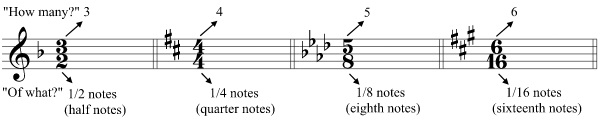
\includegraphics[width=1\textwidth]{img/timesignature}
        \caption{Meaning of the time signatures}
    \end{center}
\end{figure}

\subsection{Note / rests durations}
Both notes and rests last for certain duration, which is always a $2^n$ number of beats, where $n \in \mathbb Z$. Common values for $2^n$ are the following ones:

$$\left\{4,2,1,\frac{1}{2}, \frac{1}{4}\right\} \text{ beats}$$

Values different from these ones can be gathered through \textbf{ties} and \textbf{dots}. A dot adds $\frac{1}{2}$ the value of the note dotted, while a double dot adds $\frac{1}{2} + \frac{1}{4}$ the original value.

\subsection{Meters}
\begin{definition}[Meter]
    Describes the number of beats in a measure / bar and how they are divided.
\end{definition}

\textbf{Simple meters} break the beat into 2 parts, while \textbf{compound meters} break it into 3 parts.

They can be \textbf{double} (2 beats / bar), \textbf{triple} (3 beats / bar) or \textbf{quadruple} (4 beats / bar).

\begin{figure}[h]
    \begin{center}
        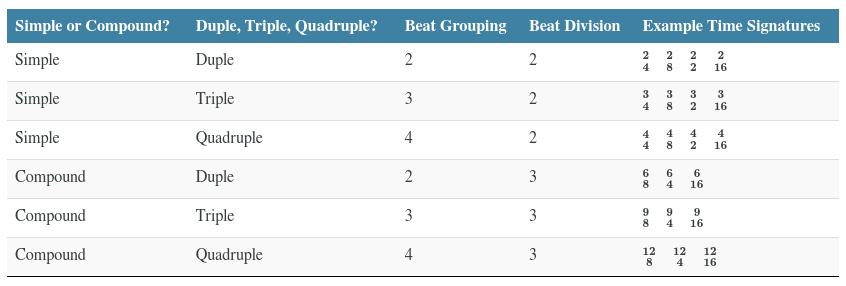
\includegraphics[width=1\textwidth]{img/meters}
        \caption{Meters}
    \end{center}
\end{figure}

The meter is traditionally identified by the time signature.

When a piece shifts between time signatures / meters often the composers employ a \textbf{metric modulation}.

\begin{definition}[Metric modulation]
    A change in tempo or subdivision, suggested by a change of meter.
\end{definition}

\subsection{Tuplets}
\begin{definition}[Tuplet]
    Rhythmic grouping of notes which would typically not occur in the specified meter.
\end{definition}

\begin{definition}[Duplet / Triplet / Quadruplet / Quintuplet]
    Common tuplet instances.
\end{definition}

\begin{definition}[Drag triplet]
    A common type of triplet, made up of quarter notes. They are called in this fashion because the rhythm seems to \emph{drag}.
\end{definition}

A drag triplet is also a common example of \textbf{hemiola}.

\begin{definition}[Hemiola (rhythm)]
    In rhythm, playing a pattern of 3 against a pattern of 2 (e.g. a drag triplet against 2 quarter notes).
\end{definition}

\subsection{Accents and syncopation}
A certain meter / time signature usually implies a certain beat hierarchy. That is, some beats are played with stronger / weaker emphases:
\begin{itemize}
    \item $4/4$: $\bullet \cdot \circ \cdot$
    \item $12/8$: $\bullet \cdot \circ \cdot$ (es. \emph{Nightmare King})
    \item $2/4$: $\bullet \cdot$
    \item $6/8$: $\bullet \cdot$ (es. \emph{White Palace}, \emph{Tarantella Napoletana})
    \item $3/4$: $\bullet \cdot \cdot$ (es. \emph{Valse di Fantastica})
    \item $9/8$: $\bullet \cdot \cdot$
    \item $3/8$: $\bullet$ (feels like 1 beat per measure)
    \item $2/2$: $\bullet \bullet$
\end{itemize}

This should also explain why some pieces are better written as $2/4$ over $4/4$: because the beat hierarchy in the measures is different.

\begin{definition}[Downbeat]
    The first beat in a measure. Usually it is played with a very strong emphasis.
\end{definition}

Through \textbf{accents}, \textbf{ties} and \textbf{rests} it is possible to alter this rhythmic framework, obtaining \textbf{syncopation} in the process.

\begin{definition}[Syncopation]
    Playing music with a stronger emphasis on the weak beats and / or a weaker emphasis on the strong beats.
\end{definition}

Through syncopation some notes can also be played on the \emph{offbeats}.

\begin{definition}[Offbeat]
    Which is not a beat.
\end{definition}

\subsection{Irregular meters}
These meters can be explained by thinking of normal meters with an uneven beat duration. That is, every measure has a fixed number of beats, but with different beat durations.

\begin{itemize}
    \item $5/4$: 5 uneven beats (es. \emph{Mars, Bringer of War}, \emph{Cinco de Chocobo})
    \begin{itemize}
        \item $3+2: \bullet \cdot \cdot \circ \cdot$
        \item $2+3: \circ \cdot \bullet \cdot \cdot$
    \end{itemize}
    \item $7/8$: 3 uneven beats (3-2-2, 2-2-3).
    \item $13/8$: 5 uneven beats (3-3-2-2-3, etc.).
\end{itemize}

\subsection{Swing}
\textbf{Swing} can be conceptualized as a way to write 6/8 in 4/4. The metronome text usually shows whether the 8th or 16th notes should be swung.

The opposite of a swing rhythm is called \textbf{straight} rhythm.

\section{Dynamics}
Dynamics hint at the volume of a given music segment. Often they range between \dynmark{ppp} and \dynmark{fff}. The intermediate dynamic \dynmark{mf} is often used as a standard base volume.

\dynmark{n} stands for \emph{niente}, and it is usually used at the end of a decrescendo.

\dynmark{fp} means to play the note as \dynmark{f}, but then quickly fade to \dynmark{p}.

\dynmark{sfz} and \dynmark{rfz} instead indicate to play a single note stronger than the surrounding ones.

\section{Control structures}
In a concert score setting often some parts do not need to play for a long number of measures. This situation is notated through a \textbf{multirest}.

\subsection{Repeats}
Repeats are sometimes highlighted with wings-like decorations, with the only purpose of making them stand out more.

\begin{definition}[Segno]
    Used as a landmark in a \textbf{D.S.} marking. \textbf{D.S.} means to play from the segno.
\end{definition}

\begin{definition}[Coda]
    Used as a landmark in a \textbf{Al coda} marking. \textbf{Al coda} means to play till the coda, then to continue playing the separate coda.
\end{definition}

Note that during a \textbf{D.C} or \textbf{D.S.} notation, repeats are \emph{not} performed for a second time.

\section{Articulations}
There a variety of articulations used to tell the player how to produce the sounds. The meaning of these often varies from instrument to instrument:

\begin{definition}[Staccato]
    Play the note short, lightly and briefly detached from the next and the previous ones.
\end{definition}

\begin{definition}[Accent]
    Emphasize the note, with a quick attack and a gentle decay / release.
\end{definition}

\begin{definition}[Marcato]
    Emphasize the note with a strong attack and a quick release / decay.
\end{definition}

\begin{definition}[Tenuto]
    The player should be careful as to keep the note for its whole duration.
\end{definition}

\begin{definition}[Staccatissimo]
    A stronger staccato.
\end{definition}

\begin{definition}[Spiccato]
    Exclusively used in string instruments. Means to lighly bounce the bow upon the strings.
\end{definition}

\begin{definition}[Portato]
    A legato-staccato. Usually means to play the notes with a light disconnection between them.
\end{definition}

\begin{definition}[Upbow \& Downbow]
    Indicates a corresponding motion of the bow on string instruments. The downbow is usually stronger.
\end{definition}

\begin{definition}[Closed / Mute \& Open]
    Usually used on percussion and brasses. These indicate whether the sound should be muted (through the \emph{sordino}, the hand, etc.) or left open to ring.
\end{definition}

\begin{definition}[Tremolo (single-note)]
    Repeat the note $2^n$ times, where $n$ is the number of strips on the stem.
\end{definition}

\begin{definition}[Tremolo (two-note)]
    Quickly alternate between the notated pitches. The actual speed of the tremolo is usually derived from context (usually: one strip $\Rightarrow$ 8th notes).
\end{definition}

\begin{definition}[Arpeggio]
    Play a series of notes in a quick sequence, but not simultaneously.
\end{definition}

\begin{definition}[Glissando]
    A quick run through all the notes between the notated ones. On piano, usually only the white notes are played.
\end{definition}

Often a glissando may be actually notated note per note, in which case it is called a \textbf{run}. Notes in a run should not be played too carefully; instead, the player should focus on the whole sequence speed.

A glissando is a \emph{discrete} change of pitch, but some instruments are able to produce a \emph{continuous} change of pitch (e.g. trombone, timpani, strings, voice).

\begin{definition}[Portamento]
    A continuous glissando.
\end{definition}
    \chapter{Scales}
    \section{Major scale}
\begin{definition}[Tetrachord]
    A 4-note scale segment with the following steps: $W-W-H$.
\end{definition}

\begin{definition}[Major scale]
    A 8-note scale made up of 2 tetrachords, joined by a whole step.
\end{definition}

$$\underbrace{W-W-H}_{T1}-W-\underbrace{W-W-H}_{T2}$$

\begin{figure}[h]
    \begin{center}
        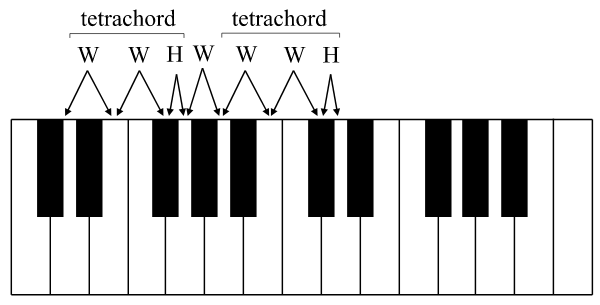
\includegraphics[width=0.6\textwidth]{img/tetrachord}
        \caption{Tetrachords in a (D) major scale}
    \end{center}
\end{figure}

A major scale uses all the 7 notes in order. No one is skipped and there are no duplicates.

\subsection{Key signatures}
There are 15 major key signatures:
\begin{itemize}
    \item 1 with no accidentals: C Major.
    \item 7 with $1$ to $7$ flats.
    \item 7 with $1$ to $7$ sharps.
\end{itemize}

\begin{figure}[h]
    \begin{center}
        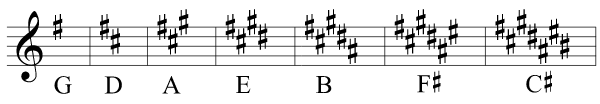
\includegraphics[width=0.8\textwidth]{img/majorsharp}
        \caption{Major key signatures (sharps)}
        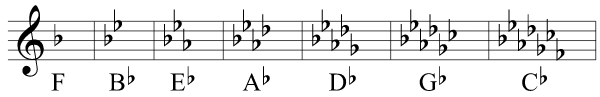
\includegraphics[width=0.8\textwidth]{img/majorflat}
        \caption{Major key signatures (flats)}
    \end{center}
\end{figure}
A key signature can be quickly identified with the following mnemonic:
\begin{itemize}
    \item With \emph{sharps}: +1 half step from the last ``sharped note''.
    \item With \emph{flats}: the second to last flat is the key (along with the flat).
\end{itemize}

\section{Minor scales}
\section{Circle of fifths}
    \chapter{Intervals}
    \section{Quantity and quality}
\begin{definition}[Harmonic interval]
    Distance between two notes played \emph{simulatenously}.
\end{definition}

\begin{definition}[Melodic interval]
    Distance between two notes played \emph{one after the other}.
\end{definition}

\begin{definition}[Interval quantity]
    The number of notes on the diatonic scale (consecutive unaltered different pitches) from the starting note to the end note.
\end{definition}

\begin{definition}[Simple intervals]
    Intervals with a quantity less than an octave.
\end{definition}

\begin{definition}[Compound intervals]
    Intervals with a quantity higher than an octave.
\end{definition}

If we talk about \emph{simple intervals}, we have some predefined quantities. Each of them has some accepted \textbf{qualities}:

\begin{center}
    \begin{tabular}{r|l}
        \textbf{Quantity} & Compatible \textbf{quantities} \\
        \hline
        Unison & Perfect \\
        Second & Major, minor \\
        Third & Major, minor \\
        Fourth & Perfect, augmented, diminished \\
        Fifth & Perfect, augmented, diminished \\
        Sixth & Major, minor \\
        Seventh & Major, minor \\
        Octave & Perfect
    \end{tabular}
\end{center}

\subsection{Multiple augmentation / diminution}
An interval can be altered through additions of subtractions of half tones.

\begin{figure}
    \begin{center}
        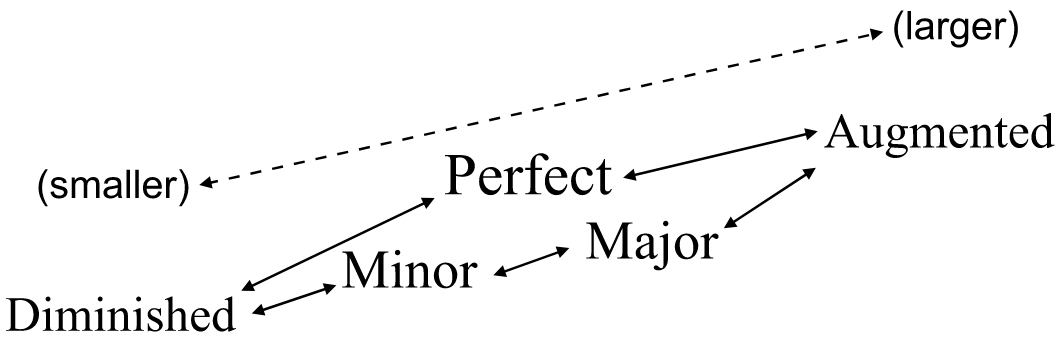
\includegraphics[width=0.8\textwidth]{img/quality}
        \caption{Interval quality chart}
    \end{center}
\end{figure}

In music notation, this is usually carried out through sharps and flats (or double sharps and double flats). From these accidentals we gather augmented / diminished intervals, but also double augmented and double augmented intervals\footnote{It is theoretically possible to reach a maximum quantity of a \emph{quintuply augmented fourth} (or \emph{quintuply diminished fifth}) by altering a tritone through a double flat - double sharp pair.}. In practice,  double augmented / double diminished intervals are rare in music, not to mention more altered quantities.

\subsection{Tritone}
Both between fifths and fourths there is a \emph{single} interval which is characterized by a much harsher sound than the others: while the others are \emph{consonant} that one is \emph{dissonant}. This interval is called the \textbf{tritone}.

\begin{definition}[Tritone]
    An augmented fourth / diminished fifth (which is always between F and B and always made up of 6 half tones or 3 whole tones - hence the name).
\end{definition}

This interval is also popularly called the \emph{diabolus in musica}, because it is the only dissonant exception to the consonant set of fourths and fifths.

Moreover, the tritone \emph{is half the width of an octave}.

\subsection{Compound intervals}
Compound intervals can be obtained by adding a 7th to an existing simple interval. Therefore, a two-octave interval is a 15th.

\subsection{Diatonic interval}
There is also a more vague type of interval, the \textbf{diatonic interval}, which essentially means: \emph{go from this note to the next one in the current diatonic scale}.

\begin{definition}[Diatonic interval]
    The distance between one note and another in the context of a specific diatonic scale.
\end{definition}

\section{Interval inversion}
An \textbf{interval inversion} can be performed by inverting the relative position of two notes, while keeping the pitch classes constant (this can be done through a single-note octave transposition).

\begin{figure}
    \begin{center}
        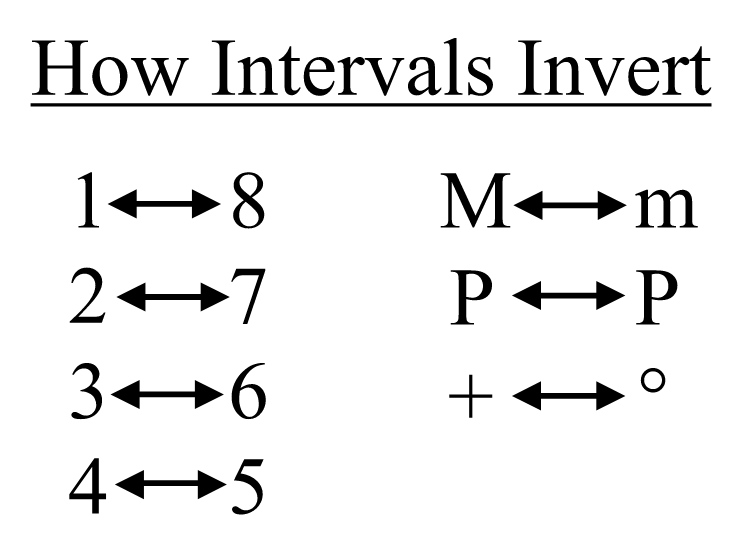
\includegraphics[width=0.4\textwidth]{img/inversion}
        \caption{Interval inversion chart}
    \end{center}
\end{figure}

As we can see, the sum of an interval quantity with the quantity of its inverted counterpart is always 9. Moreover:
\begin{itemize}
    \item Perfect intervals invert to perfect intervals.
    \item Augmented invervals invert to diminished intervals.
    \item Major intervals invert to minor intervals.
\end{itemize}
    \chapter{Pitch}
    \section{Sound properties}
A \textbf{sound} is just a bunch of air particles which vibrate really quickly into thin air. They do so on \emph{longitudinal} waves. The vibration in the air is produced by some sort of vibrating device (e.g. the membrane of a PC speaker) and captured by some other device (like the membranes into our ears). In the case of our ears, the brain processes the captured vibrations into sound perceptions.

The number of vibrations per second is expressed through the \textbf{frequency} $f$, expressed in \emph{Hertz}. Higher frequencies produce higher sounds. Conversely, if the signal has a bigger \textbf{amplitude} it is perceived as a louder sound. The timbre is instead related to the overall waveform shape and therefore to the Fourier representation of the signal.

Therefore, to summarise:
\begin{itemize}
    \item \textbf{Frequency} translates to \textbf{pitch}.
    \item \textbf{Amplitude} translates to \textbf{volume}.
    \item \textbf{Waveform shape} translates to \textbf{timbre}.
\end{itemize}

\section{Pitch}
Unfortunately, the relationship between frequency and pitch is nonlinear. In fact, it is \emph{exponential}.

Moving in octaves (in pitch space) to us feels like a linear increase, while in frequency the same movement is exponential (or also, the frequency increase is linear, but the pitch increase is logarithmic). As an example moving a sound to the next note involves \emph{doubling} its frequency.

Therefore, if we express as $s$ the multiplicative factor used to scale the frequency so as to obtain the corresponding pitch raised by a semitone:

$$s^{12} = 2 \Rightarrow s = 2^{\frac{1}{12}}$$

For translating a given pitch into a frequency we can use the following:

$$f = f_\textbf{C0} \cdot 2^{o+\frac{p}{12}}$$

Where $p$ is the number of semitones from the $C$ pitch class and $o$ is the number of octaves.

The reverse can be computed through logarithms and fixed / fractional part functions.

Nevertheless, from this we gather a pretty interesting result: \textbf{the pitch we perceive as a linear increase translates in reality as an exponential increase in frequency}.

This means that the most interesting octaves in music (C0 - C10) are effectively translated to a very narrow set of frequencies, up to 1000 Hz.

\subsection{Pitch class and octave equivalence}
The set of C pitches is called the \emph{C pitch class}. This can be generalized.

\begin{definition}[Pitch class]
    A pitch without its octave.
\end{definition}

We recognize pitches which share the same pitch class as different instances of the same note. In fact, these pitches are $n$ octaves apart so we should say that we recognize pitches \emph{which are $n$ octaves apart} as different instances of the same note.

Why is this so? This is because the waveforms of two notes from an octave interval perfectly line up together.

If we make an equivalence relation out of the notion of \emph{pitch space modulo octave equivalence} we are able to obtain the \textbf{pitch class space}.

\subsection{Temperament}
The modern western musical system is said to be a \textbf{12-tone equal-tempered} one.

\begin{definition}[12-tone equal-temperament]
    A musical system in which an octave is subdivided into a set of 12 equal semitones (equal = there is a constant amount between every semitone in pitch space).
\end{definition}

However, more than two centuries ago, composers actually used systems which were not equally-tempered. The semitones had different sizes across the octave, therefore leading to uneven intervals, be it for the better or for the worse. In fact, some of these intervals sound \emph{better} than their equally-tempered counterparts; however, these intervals lead to inconsistencies into other intervals / parts of the octave, which sound drastically worse than their equally-tempered counterparts (these intervals were called \textbf{wolf intervals}).
\end{document}